\documentclass[tikz,border=3.14mm]{standalone}
\usetikzlibrary{calc,patterns}

\begin{document}

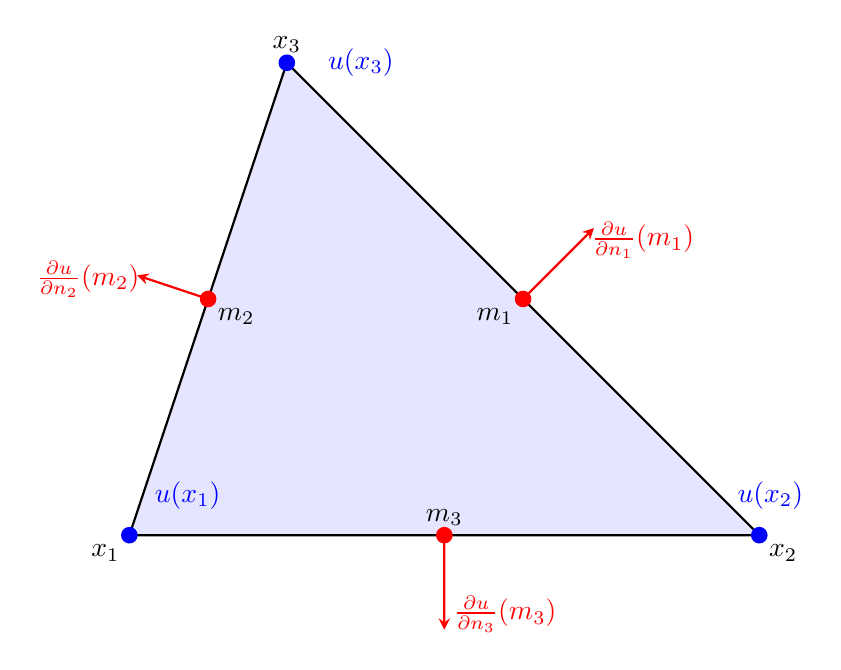
\begin{tikzpicture}[scale=2,>=stealth]

    % 定义三角形顶点
    \coordinate (A) at (0,0);
    \coordinate (B) at (4,0);
    \coordinate (C) at (1,3);
    
    % 绘制三角形单元
    \draw[thick,fill=blue!10] (A) -- (B) -- (C) -- cycle;
    
    % 标记顶点
    \node[below left] at (A) {$x_1$};
    \node[below right] at (B) {$x_2$};
    \node[above] at (C) {$x_3$};
    
    % 标记边中点
    \coordinate (M12) at ($(A)!0.5!(B)$);
    \coordinate (M23) at ($(B)!0.5!(C)$);
    \coordinate (M31) at ($(C)!0.5!(A)$);

    \node[above] at (M12) {$m_3$};
    \node[below left] at (M23) {$m_1$};
    \node[below right] at (M31) {$m_2$};
    
    % 在边中点绘制点并标记法向导数
    \fill[red] (M12) circle (1.5pt);
    \fill[red] (M23) circle (1.5pt);
    \fill[red] (M31) circle (1.5pt);
    
    % 绘制顶点
    \fill[blue] (A) circle (1.5pt);
    \fill[blue] (B) circle (1.5pt);
    \fill[blue] (C) circle (1.5pt);

    % 绘制法向量(垂直于边向外)
    \draw[->,red,thick] (M12) -- ($(M12)!0.3!90:(A)$);
    \draw[->,red,thick] (M23) -- ($(M23)!0.3!90:(B)$);
    \draw[->,red,thick] (M31) -- ($(M31)!0.3!90:(C)$);
    
    % 标记法向导数
    \node[red,right] at ($(M12)!0.5!($(M12)!0.5!90:(A)$)$) {$\frac{\partial u}{\partial n_3}(m_3)$};
    \node[red,right] at ($(M23)!0.5!($(M23)!0.5!90:(B)$)$) {$\frac{\partial u}{\partial n_1}(m_1)$};
    \node[red,left] at ($(M31)!0.5!($(M31)!0.5!90:(C)$)$) {$\frac{\partial u}{\partial n_2}(m_2)$};
    
    % 标记顶点函数值
    \node[blue,above right] at ($(A)+(0.1,0.1)$) {$u(x_1)$};
    \node[blue,above right] at ($(B)+(-0.2,0.1)$) {$u(x_2)$};
    \node[blue,right] at ($(C)+(0.2,0)$) {$u(x_3)$};

\end{tikzpicture}

\end{document}